\myframe{CEA project: \hfill  determinacy in a real-time kernel}
{
  \hspace{-18pt}{\color{Maroon} The Problem:} \\

  \vspace{50pt}


}

\myframe{CEA project: \hfill  no errors}
{
\begin{center}
\includegraphics[scale=0.32]{cea1.png}
\end{center}
}

\myframe{CEA project: \hfill  error at time 4}
{
\begin{center}
\includegraphics[scale=0.32]{cea2.png}
\end{center}
}

\myframe{CEA project: \hfill error in time window}
{
\begin{center}
\includegraphics[scale=0.32]{cea3.png}
\end{center}
}


% Real time kernel which interleaves concurrent processes on a single CPU.
% processes communicate via messages (what ever that means right now).
% Want to guarantee that each process computes the same result, no matter how 
% they got interleaved (Determinacy).


\myframe{CEA project: \hfill determinacy in a real-time kernel}
{
\scriptsize
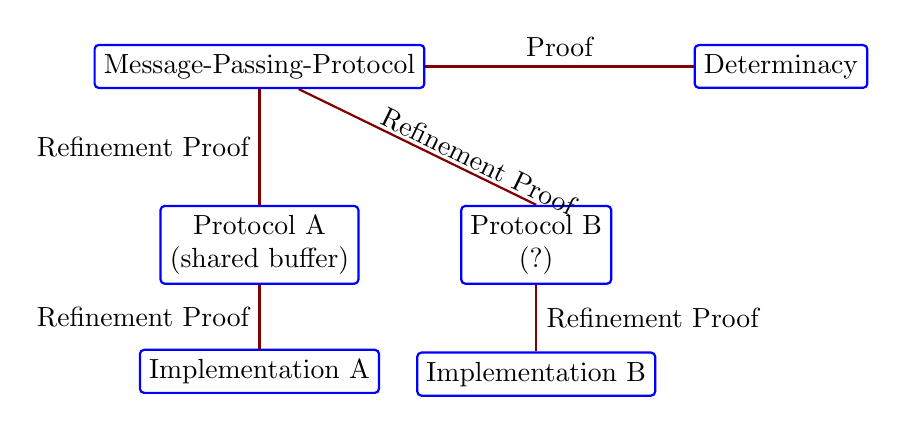
\begin{tikzpicture}[thick, main node/.style={rectangle, draw=Blue, rounded corners=1.5, align=center}]
\node[main node] (0) [ ] {Message-Passing-Protocol}; 

\node[main node] (1) [right of=0, xshift=160pt] {Determinacy};

\node[main node] (2) [below=0, yshift=-50pt] {Protocol A\\(shared buffer)};

\node[main node] (3) [below=0, yshift=-50pt, xshift=100pt] {Protocol B\\ (?) };

\node[main node] (4) [below=2, yshift=-100pt] {Implementation A};

\node[main node] (5) [below=3, yshift=-100pt, xshift=100pt] {Implementation B};

\path[]
 (0.east)   edge [draw=Maroon] node [above] {Proof} (1.west)
 (0.south)  edge [draw=Maroon] node [left] {Refinement Proof} (2.north)
 (0.330)    edge [draw=Maroon] node [right, sloped, yshift=5pt, xshift=-20pt] {Refinement Proof} (3.north)
 (2.south)  edge [draw=Maroon] node [left] {Refinement Proof} (4.north)
 (3.south)  edge [draw=Maroon] node [right] {Refinement Proof} (5.north)
;

        

\end{tikzpicture}
}

% Diagram:
% Abstract spec of a message passing protocol + proof of Determinacy,
% + proofs that two different protocols (shared buffer + ?) implement that spec
% + proofs that C-code implements those protocols (blue sky thinking is allowed :-))

% TLA code snipplets
